\section{An\'alisis del m\'etodo Moreno-Dominguez}
\label{sec:analisis_moreno}

El cuarto paso del diagrama en la figura \ref{fig:diagrama} es agrupar los
tractogramas mediante un algoritmo de $clustering$. Moreno-Dominguez et
al. \cite{Moreno-Dominguez2014} implementan el algoritmo
\textit{Agglomerative Hierarchical Clustering} para agrupar los
tractogramas. En particular utilizan como medida de similitud la distancia
coseno (ecuaci\'on \ref{eq:cosine}) y como criterio de \textit{linkage} el
centroide (ecuaci\'on \ref{eq:centroide}). Utilizar \textit{Hierarchical
Agglomerative Clustering} con la distancia coseno y el \textit{linkage}
centroide presenta algunas desventajas. Primero, la distancia coseno no
distingue distancias entre clusters colineales. Segundo, el promedio de
probabilidades no necesariamente representa una probabilidad 
\cite{Pohl2007}. Esto quiere decir que el centroide de un grupo de
tractogramas no necesariamente representa el promedio de estos
tractogramas. Finalmente la distancia coseno obliga a tener que comparar
expl\'icitamente cada centroide con los clusters existentes. Esto aumenta
la complejidad temporal y espacial ya que es necesario mantener los
tractogramas en memoria. A continuaci\'on detallamos cada una de estas
desventajas. \\

\subsection{Clustering de vectores colineales}

La distancia coseno (ecuaci\'on \ref{eq:cosine}) es una forma de medir 
correlaci\'on entre vectores. Supongamos tenemos
vectores aleatorios colineales donde cada componente es independiente y 
proviene de una distribuci\'on de Bernulli. Agruparlos utilizando como
medida de similitud la distancia coseno lleva a resultados err\'oneos. 
Por ejemplo, agrupar los puntos de la figura \ref{fig:3clusters} usando
el m\'etodo de Moreno-Dominguez da como resultado la figura 
\ref{fig:3moreno}. Podemos ver que si bien ten\'iamos tres clusters bien
definidos en el espacio el m\'etodo no logr\'o separarlos. \\

\begin{figure}[h!]
        \centering
        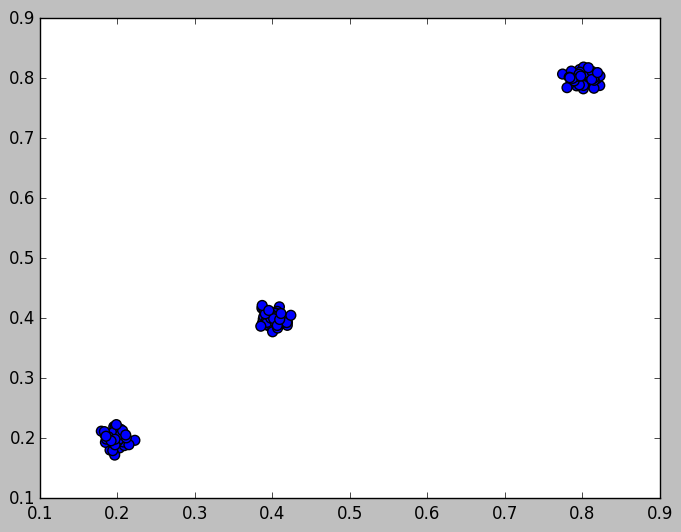
\includegraphics[width=0.5\textwidth]{img/3pop.png}
        \caption{Tres $clusters$ colineales. Cada punto representa un
                 vector aleatorio con componentes provenientes de una
                 distribucion Bernulli. Queremos agruparlos utilizando
                 \textit{Agglomerative Hierarchical Clustering}.}
        \label{fig:3clusters}
\end{figure}

Tambi\'en existe otro problema. Por la forma que posee el algoritmo 
\ref{alg:itract}, los tractogramas creados poseen muchos voxels lejanos
con valores peque\~nos. El algoritmo simula el recorrido de part\'iculas de
agua sobre mapas de transiciones probabil\'isticas. Cuanto mas lejano un 
voxel mayor cantidad de transiciones se necesitan para llegar. Por lo 
tanto, cuanto mas lejos se encuentra un voxel, menor probabilidad tiene de
ser visitado. Para visualizar esto mejor situamos semillas en el \'area
de Broca de un sujeto y generamos sus tractogramas. La figura 
\ref{fig:hist_tract} muestra el histograma de los valores en los mapas de
visitas. Cada voxel dentro de un mapa de visitas indica que cantidad de 
part\'iculas pasaron por \'el.
En este caso el $70\%$ de los voxels visitados fueron alcanzados por solo
una part\'icula. Esta gran cantidad de voxel con valores tan bajos podr\'ia
generar ruido en las correlaciones. \\

\begin{figure}[h!]

\centering                                                                                                          
\begin{minipage}[b]{0.85\textwidth}
    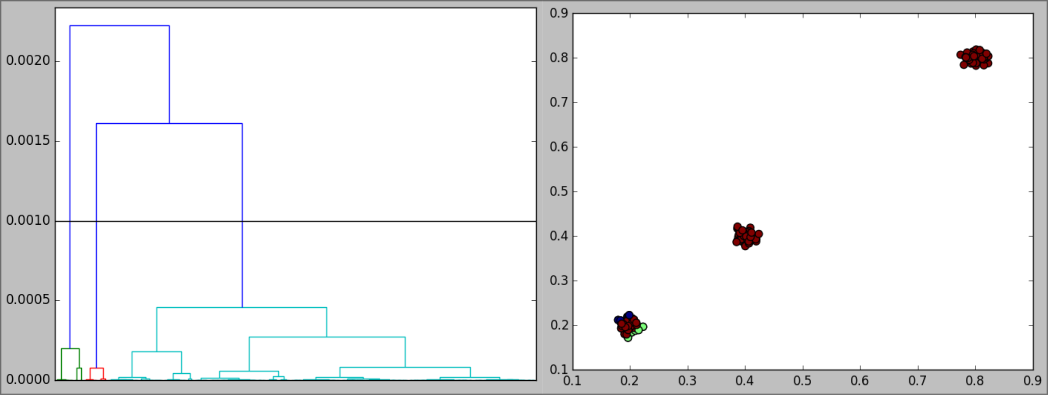
\includegraphics[width=\textwidth]{img/3pop_moreno.png}
    \caption{$Clustering$ resultante de utilizar el m\'etodo de 
             Moreno-Dominguez para agrupar los vectores. El algoritmo
             agrupa la mayor\'ia de los vectores en una \'unica 
             categor\'ia.}
    \label{fig:3moreno}
\end{minipage} ~

\end{figure}  

\begin{figure}[h!]
              \centering                                                                                                          
\begin{minipage}[b]{0.8\textwidth}
    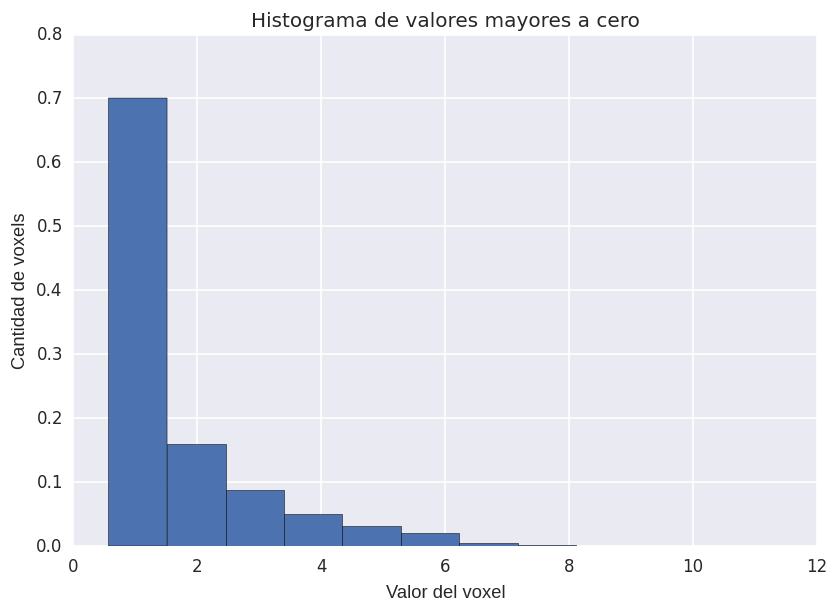
\includegraphics[width=\textwidth]{img/hist_tract.png}
    \caption{Histograma normalizado de los valores en los mapas de visitas
             del \'area de Broca. No se muestran los valores mayores a 12.
             La mayor parte de los voxels visitados tuvieron una \'unica
             visita.}
    \label{fig:hist_tract}
\end{minipage} ~

\end{figure}  


\subsection{Relaci\'on m\'etrica-\textit{linkage}}

Moreno-Dominguez et al. utilizan como medida de similitud la distancia
coseno (ecuaci\'on \ref{eq:cosine}) y como criterio de \textit{linkage} el
centroide (ecuaci\'on \ref{eq:centroide}). La medida de similitud 
compara el \'angulo de los vectores, pero el $linkage$ crea un 
representante minimizando la distancia eucl\'idea a ambos clusters. No
parecieran ser compatibles. Veamos un ejemplo. La figura \ref{fig:cos_cen}
muestra 4 vectores aleatorios $p_i = (X_i, Y_i)$. Las variables $X_i$ e
$Y_i$ son independientes y provienen de una distribuci\'on Bernulli. Las
posiciones en coordenadas polares de cada vector son: 
$ p_1 = (0.4, 45^\circ)$; $p_2 = (0.3, 25^\circ)$; $p_3 = (0.4, 66^\circ)$
y $p_4 = (0.4, 4.5^\circ)$. \\

\begin{figure}[h!] 
    \centering
    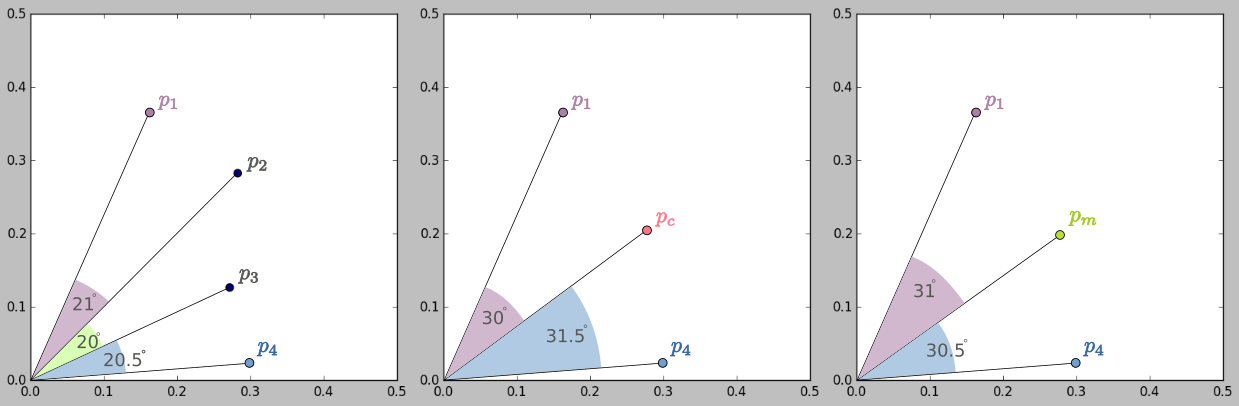
\includegraphics[width=\textwidth]{img/cosine_centroid.png}
    \caption{El centroide ($p_c$) de $p_2$ y $p_3$ no representa el punto
             medio ($p_m$) respecto al \'angulo entre ellos.}
    \label{fig:cos_cen}
\end{figure} 

Podemos apreciar que al principio $d(p_2,p_3) < d(p_3,p_4) < d(p_1,p_2)$,
siendo $d(x,y)$ la distancia coseno (ecuaci\'on \ref{eq:cosine}). Sin
embargo, luego de utilizar el \textit{linkage centroid} 
(ecuaci\'on \ref{eq:centroide}) sucede que $d(p_1,p_c) < d(p_4,p_c)$. $p_4$
es ahora el punto que mas lejos est\'a del centroide. Creando un
representante $p_m$ usando el \'angulo medio entre $p_2$ y $p_3$ esto no
sucede. Este fen\'omeno se da porque la distancia coseno tiene en cuenta
el \'angulo pero el centroide no. Por lo tanto el centroide no caracteriza
al punto medio respecto a la distancia coseno. \\


\subsection{Complejidad algor\'itmica del clustering}
\label{sec:complejidad_moreno}

El diagrama de la figura \ref{fig:diagrama} divide el proceso de 
parcelaci\'on de la corteza en varios pasos: seleccionar los voxels que 
ser\'an utilizados como semilla de cada tractograma; luego generar cada
tractograma y finalmente agruparlos usando alg\'un algoritmo de clustering.
En todo este proceso el paso mas caro en t\'erminos computacionales es el
\textit{clustering}. Veamos la  complejidad del m\'etodo propuesto por
Moreno-Dominguez. En cada iteraci\'on del algoritmo es necesario calcular
un centroide, almacenarlo y compararlo expl\'icitamente con el resto de
los clusters. Por cada iteraci\'on es necesario hacer 
$O(c^2 m)$ operaciones para recalcular todas las distancias, donde $c$ es
la cantidad de clusters y $m$ es la longitud de los mismos. Dadas $s$
semillas iniciales, la cantidad de iteraciones a realizar son $s-1$. La
complejidad temporal de este m\'etodo es $O(s^3 m)$. Respecto a la 
complejidad espacial, el mantener todos los clusters en memoria requiere
$O(s m)$ espacio. Tambi\'en es necesario mantener la matriz de distancias
entre $clusters$, la cual requiere $O(s^2)$. La complejidad espacial total
es $O(s m + s^2)$. Podemos notar que ambas complejidades dependen de $m$.
\\ 

Resumiendo, utilizar \textit{Hierarchical Agglomerative Clustering} 
con la distancia coseno y el \textit{linkage} centroide presenta algunas
desventajas: La medida de similitud y el $linkage$ no son compatibles;
no permite agrupar de manera correcta clusters colineales y 
necesita mantener todos los $clusters$ en memoria as\'i como tambi\'en
compararlos expl\'icitamente. \\
